\documentclass{article}

% Top margin, right margin, left margin, bottom margin, footnote skip
\usepackage[utf8]{inputenc}
\usepackage{biblatex}
\addbibresource{./references.bib}
% linktocpage shall be added to snippets.
\usepackage{hyperref,theoremref}
\hypersetup{
	colorlinks, 
	linkcolor={red!40!black}, 
	citecolor={blue!50!black},
	urlcolor={blue!80!black},
	linktocpage % Link table of content to the page instead of the title
}

\usepackage{blindtext}
\usepackage{titlesec}
\usepackage{amsthm}
\usepackage{thmtools}
\usepackage{amsmath}
\usepackage{amssymb}
\usepackage{graphicx}
\usepackage{titlesec}
\usepackage{xcolor}
\usepackage{multicol}
\usepackage{hyperref}
\usepackage{import}
\usepackage{libertinus}           % Load the Libertinus font
\usepackage{mathbbol}
\usepackage{bm}
\usepackage{mathrsfs}

\usepackage{tikz}
\usepackage{tikz-cd}
\usetikzlibrary{arrows.meta, positioning}
% \usepackage{calrsfs}


\newtheorem{theorem}{Theorem}[section]
\newtheorem{lemma}[theorem]{Lemma}
\newtheorem{corollary}{Corollarium}[section]
\newtheorem{proposition}{Proposition}[theorem]
\theoremstyle{definition}
\newtheorem{definition}{Definition}[section]

\theoremstyle{definition}
\newtheorem{axiom}{Axioma}[section]

\theoremstyle{remark}
\newtheorem{remark}{Remark}[section]
\newtheorem{hypothesis}{Coniectura}[section]
\newtheorem{example}{Exampli Gratia}[section]
% Proof Environments
\newcommand{\thm}[2]{\begin{theorem}[#1]{}#2\end{theorem}}

% \renewenvironment{proof}{{\bfseries\emph{Demonstratio.}}}{\qed}
\renewcommand\qedsymbol{Q.E.D.}

\newcommand{\D}{\bm{\Delta}}
\renewcommand{\S}{\textbf{Set}}
\newcommand{\sS}{\textbf{sSet}}
\newcommand{\op}{^{\text{op}}}
\newcommand{\N}{\mathbb{N}}
\renewcommand{\L}{\Lambda}

\let\H\relax
\DeclareMathOperator{\H}{\text{Hom}}


\renewcommand{\emph}{\textbf}

\title{$\infty$-Category and Simplicial Sets}
\author{Candidate Number: 1099144} 
\date{\today}

\begin{document}
\maketitle

\tableofcontents

\section{Simplicial Category and Simplicial Sets}

\subsection{Definition of Simplical Sets}

The goal of this mini-project to to define $\infty$-categories via simplicial sets. 
The definition of simplicial sets is based on the \emph{simplex category}, $\D$.

\begin{definition}[Simplex Category \cite{lurie}]
	The \emph{simplex category}, denoted as $\D$, is defined as
	\begin{enumerate}
		\item Its objects linearly ordered finite sets $[n] = \{0 < 1 < \cdots < n\}$ for all $n \geq 0$.
	\item Its morphisms are given by order-preserving maps.
	\end{enumerate}
	Simplex category is also known as the category of combinatorial simplices
\end{definition}

It is clear that $\D$ is equivalent to the category of all finite non-empty totally ordered sets with order-preserving maps. 

For each $n, j \in \N, 0\leq j \leq n$, define \emph{face} and \emph{degenerate} maps repectively as $\D$, $d^{j,n}: [n - 1] \to [n]$ and $s^{j, n}: [n + 1] \to [n]$ given by
\begin{equation}
	d^{j, n}(i) = \begin{cases}
		i & i < j \\
		i + 1 & i \geq j
	\end{cases}, \quad
	s^{j,n}(i) = \begin{cases}
		i & i \leq j \\
		i - 1 & i > j
	\end{cases}.
\end{equation}

Concretely, the face map $d^{j, n}$ is the only injective and order-preserving maps from $[n - 1]$ to $[n]$ that misses $j \in [n]$, and the degenerate map $s^{j, n}$ is the only surjective and order-preserving map from $[n + 1]$ to $[n]$ that hits $j \in [n]$ twice.

Since the domain and codomain of the face and degenerate maps will always be clear from the context, we will drop the superscripts and denote them as $d^j$ and $s^j$.

Let $i < j$. 
The composition of face maps $d^jd^i$ is the unique injective and order-preserving map from $[n - 2]$ to $[n]$ that misses both $i$ and $j \in [n]$. 
A moment of thought shows that this map is the same as $d^id^{j - 1}$.
There are similar relations for the compositions of degenerate maps and mixed compositions of face and degenerate maps. 
All of the identities are listed below.

% TODO: check the middle case
\begin{align}
	d^jd^i &= d^id^{j - 1}, \quad i < j \label{sim1} \\
	s^js^i &= s^is^{j + 1}, \quad i \leq j  \label{sim2} \\
	s^j d^i &= \begin{cases}
		d^i s^{j - 1} & j < i \\
		\text{id} & j = i, i + 1 \\
		d^{i - 1} s^j & j > i + 1
	\end{cases} \label{sim3}
\end{align}

It can be shown that all morphisms in $\D$ can be generated by compositions of face and degenerate maps.

We are now ready to define simplicial sets.

\begin{definition}[Simplicial Set \cite{lurie}]
	A \emph{simplicial set} is presheaf on $\D$, i.e.,
	a functor $X: \D\op \to \S$. 
	We will denote the category of simplicial sets as $\sS$.
\end{definition}

Let $X$ be a simplicial set.
Define $X_n := X([n])$.
We shall define the face map $d_j: X_n \rightarrow X_{n-1}$ as the map induced by the face map on $\D$, $d^j: [n - 1] \to [n]$. 
That is $d_j = Xd^j$. 
Similarly, denote $s_j: X_n \to X_{n + 1}$ the map induced by the degenerate map $s^j: [n + 1] \to [n]$, i.e., $s_j = Xs^j$.
Since $X$ is contravariant, $d_j$ and $s_j$ will satify the following identities, reversing the order of composition compared to \eqref{sim1}, \eqref{sim2}, and \eqref{sim3}. 

\begin{align}
	d_i d_j &= d_{j - 1} d_i, \quad i < j \label{simp1} \\
	d_i s_j &= \begin{cases}
		s_{j - 1} d_{i} & j < i \\
		\text{id} & j = i, i + 1 \\
		s_{j} d_{i - 1} & j > i + 1
	\end{cases} \label{simp3} \\
	s_i s_j &= s_{j + 1} s_i, \quad i \leq j  \label{simp2} 
\end{align}

Since $d^j$ and $s^j$ generates all morphisms in $\D$, the morphisms $d_j$ and $s_j$ will generate all relevant morphisms in $\S$ relevant to $X$ (Recall $X \in [\D\op, \S]$). 
This gives a crucial observation. 

\begin{remark}\label{sim-set-data}
The data given by a simplicial set $X$ is equivalent to the data of a sequence of sets $\{X_n\}_{n \geq 0}$ together with face and degenerate maps $d_j: X_n \to X_{n - 1}$ and $s_j: X_n \to X_{n + 1}$ satisfying the identities \eqref{simp1}, \eqref{simp2}, and \eqref{simp3}.
\end{remark}

\subsection{Horn and Simplices}

The first intuitive example of simplicial sets are the standard simplices, which are the Yoneda embeddings of the objects in $\D$.

\begin{definition}[Standard n-Simplex \cite{lurie}]
	For each $n \geq 0$, the \emph{standard n-simplex} is, denoted as $\Delta^n$, is the Yoneda embedding of $[n] \in \D$, i.e., 
	\begin{equation*}
		\Delta^n := \H_{\D}(-, [n]): \D\op \to \S.
	\end{equation*}
	$\D^n$ is a simplicial set, because $\H(-, A)$ can be regarded as a contravariant functor to the $\S$ of morphisms.
\end{definition}

Another important class of simplicial sets are horns, which can be thought of as simplices with one face missing.

\begin{definition}[Horn \cite{lurie}]
	For each $n \geq 1$ and $0 \leq i \leq n$, the \emph{$i$-th horn}, denoted as $\L^n_i$, is the simplicial defined as
	\begin{enumerate}
		\item $\L^n_i([m]) = \{f \in \H_{\D}([m], [n]) : [n] \smallsetminus \{i\} \not\subseteq f([m])\}$. 
			In other words, $\L^n_i ([m])$ is the set of all order-preserving maps from $[m]$ to $[n]$ that miss at least one element in $[n] \smallsetminus \{i\}$.
		\item For a map $s \in \H_{\D} ([m], [k])$, the corresponding map $\L^n_i(s): \L^n_i[k] \rightarrow \L^n_i[m]$ are its pullback (see Figure \ref{fig:horn-pullback}), i.e., for $f \in \L^n_i [k]$ , 
			$$
				\L^n_i(s) (f) = f \circ s
			$$
	\end{enumerate}
	Moreover, $\L^n_i$ is called an \emph{inner horn} if $0 < i < n$, and an \emph{outer horn} if $i = 0$ or $i = n$.
\end{definition}

\begin{figure}
	\centering
	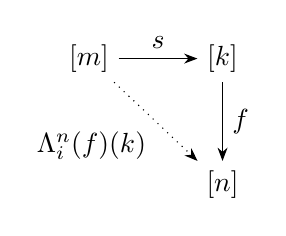
\begin{tikzpicture}[->, >=Stealth]
  % Nodes
	\node (A) {$[m]$};
	\node[right=of A] (B) {$[k]$};
	\node[below=of B] (C) {$[n]$};

  % Arrows (legs of the right triangle)
  \draw (A) -- node[above] {$s$} (B);
  \draw (B) -- node[right] {$f$} (C);

  \draw[dotted] (A) -- node[below left] {$\L^n_i(f) (k)$} (C);
\end{tikzpicture}
\caption{Pullback defining the map $\L^n_i(s): \L^n_i[k] \rightarrow \L^n_i[m]$}
\label{fig:horn-pullback}
\end{figure}

$\L^n_i [m]$ is a functor from $\D\op$ to $\S$ by the standard arguments of pullback.
Because $f \in \L^n_i[k]$, it misses at least one element in $[n] \smallsetminus \{i\}$, so must $f \circ s$.
Therefore the requirement that $\L^n_i(s) (f) \in \L^n_i [m]$ is satisfied, and the definition is self-consistent.



\newpage
\printbibliography

\end{document}
